\documentclass[brazil]{beamer}
\usepackage{beamerthemesplit}
\usepackage[brazilian]{babel}
\usepackage[utf8]{inputenc}
\usepackage{color}
\usepackage{xcolor}
\usepackage{graphicx}
%\usepackage{subcaption}
\usepackage{float}
\usepackage{wrapfig}
\usepackage{amssymb}
\usepackage{amsmath}
\usepackage{fancybox}
\usepackage{ulem}
\usepackage{listings}
\usepackage{upquote}
\setbeamertemplate{footline}[frame number]
\usetheme{Dresden}

%http://tex.stackexchange.com/questions/100838/beamer-dresden-theme-miniframes-appeareance-and-frame-number-insertion
\newcommand{\frameofframes}{/}
\newcommand{\setframeofframes}[1]{\renewcommand{\frameofframes}{#1}}
\setframeofframes{of}
\makeatletter
\setbeamertemplate{footline}
  {%
    \begin{beamercolorbox}[colsep=1.5pt]{upper separation line foot}
    \end{beamercolorbox}
    \begin{beamercolorbox}[ht=2.5ex,dp=1.125ex,%
      leftskip=.3cm,rightskip=.3cm plus1fil]{author in head/foot}%
      \leavevmode{\usebeamerfont{author in head/foot}\insertshortauthor}%
      \hfill%
      {\usebeamerfont{institute in head/foot}\usebeamercolor[fg]{institute in head/foot}\insertshortinstitute}%
    \end{beamercolorbox}%
    \begin{beamercolorbox}[ht=2.5ex,dp=1.125ex,%
      leftskip=.3cm,rightskip=.3cm plus1fil]{title in head/foot}%
      {\usebeamerfont{title in head/foot}\insertshorttitle}%
      \hfill%
      {\usebeamerfont{frame number}\usebeamercolor[fg]{frame number}\insertframenumber~\frameofframes~\inserttotalframenumber}
    \end{beamercolorbox}%
    \begin{beamercolorbox}[colsep=1.5pt]{lower separation line foot}
    \end{beamercolorbox}
  }
\makeatother

\usefonttheme{structurebold}

\begin{document}

  \title{Metaballs no PBRT}
  \author{Vinícius Vendramini e Wilson Kazuo Mizutani}

  \frame{
    \titlepage
  }
  
  \section{Introdução}
  
    \subsection{}
    \begin{frame}
      \frametitle{Metaballs}
      \begin{columns}
        \begin{column}{0.58\textwidth}
          \begin{itemize}
            \item Objetos de aparência orgânica
            \item Difícil de modelar manualmente e de extrair da natureza
            \item Comumente usadas para fluidos, fumaça, eletrosferas e imagens médicas
          \end{itemize}
        \end{column}
        \begin{column}{0.4\textwidth}
          \begin{center}
            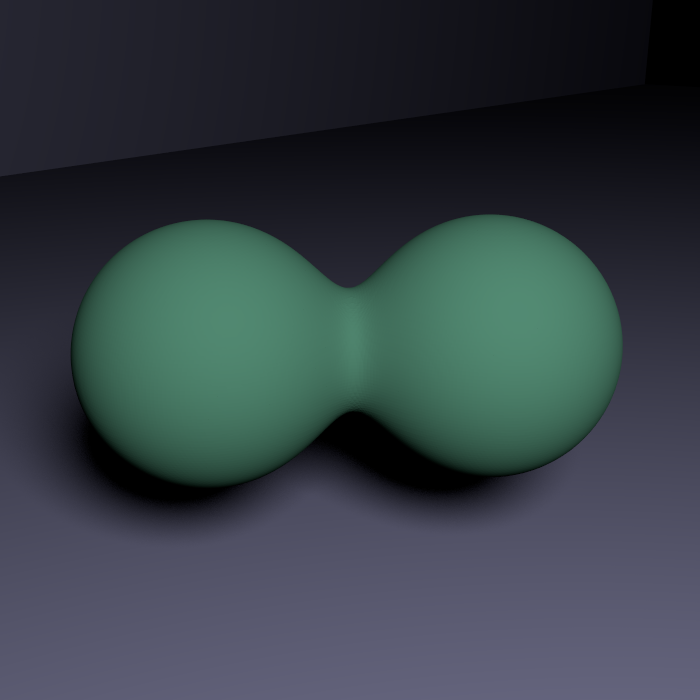
\includegraphics[width=1.0\textwidth]{imgs/metaball-good1.png}
          \end{center}
        \end{column}
      \end{columns}
    \end{frame}

    \begin{frame}
      \frametitle{Metaballs}
      \begin{itemize}
        \item Definidas de forma geral no $\mathbb{R}^n$
        \item Aqui com $F:\mathbb{R}^3 \to \mathbb{R}$
        \vspace{.5em}
        \begin{center}
          $F(x) = D(x) - T$
        \end{center}
        \begin{itemize}
          \item $T$: threshold
          \item $D(x)$: soma das exponenciais
            \vspace{-1.0em}
            \begin{center}
              $$D(x) = \sum_{i = 1}^n Te^{\frac{B_i}{R_i^2}||x-P_i||^2-B_i} $$
            \end{center}
          \item $B_i$: Blobbiness
          \item $R_i$: Raio
        \end{itemize}
      \end{itemize}
    \end{frame}
      
    \begin{frame}
      \frametitle{Metaballs}
        \begin{center}
          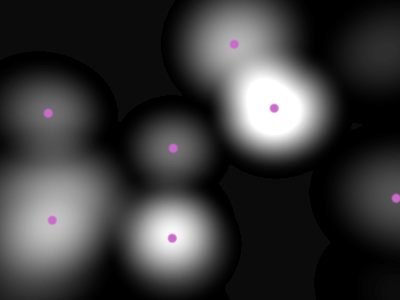
\includegraphics[width=.7\textwidth]{imgs/metaball-2d-1.png}
        \end{center}
    \end{frame}

    \begin{frame}
      \frametitle{Metaballs}
        \begin{center}
          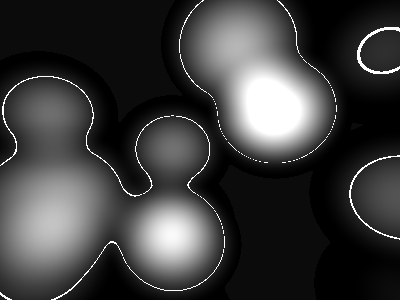
\includegraphics[width=.7\textwidth]{imgs/metaball-2d-2.png}
        \end{center}
    \end{frame}

    \begin{frame}
      \frametitle{Metaballs}
        \begin{center}
          
\includegraphics[width=.7\textwidth]{imgs/metaball-2d-3.png}
        \end{center}
    \end{frame}

    % Efeito dos parâmetros

  \section*{Implementação Analítica}
    \subsection{}
        
    \begin{frame}
      \frametitle{Physically Based Ray Tracer}
      \begin{itemize}
        \item Ray Tracer didático
        \item Subclasses da classe \textbf{Shape}
        \item Intersectable vs. non-intersectable
        \item Cálculos de intersecção
      \end{itemize}
    \end{frame}    

    \begin{frame}
      \frametitle{Algoritmo de Blinn}
      \begin{itemize}
        \item A equação das metaballs não tem solução analítica:
          \vspace{-1.0em}
          \begin{center}
            $$D(x) = \sum_{i = 1}^n Te^{\frac{B_i}{R_i^2}||x-P_i||^2-B_i} $$
          \end{center}
          \vspace{.5em}
        \item Iteração de Newton
        \item Regula-falsi
      \end{itemize}
    \end{frame}

    \begin{frame}
      \frametitle{Iteração de Newton}
      \begin{itemize}
        \item Achar o $t_{next}$ dado um $t^*$:
          \vspace{0.5em}
          \begin{center}
            $$ t_{next} = t^* - \frac{D(t^*) - T}{D'(t^*)} $$
          \end{center}        
        \item $t_{next}$ pode divergir
        \item É relativamente rápido
      \end{itemize}
    \end{frame}

    \begin{frame}
      \frametitle{Regula-falsi}
      \begin{itemize}
        \item Achar o $t_{next}$ entre $t_0$ e $t_1$:
          \vspace{0.5em}
          \begin{center}
            $$ t_{next} = \frac{t_0(D(t_1) - T) - t_1(D(t_0) - T)}{D(t_1) - D(t_0)} $$
          \end{center}        
        \item Sempre converge para a solução
        \item É relativamente lento
        \item Solução: alternar entre um e outro.
      \end{itemize}
    \end{frame}    

    \begin{frame}
      \frametitle{Arquitetura do PBRT}
      \begin{itemize}
        \item Precisa de geometria diferencial
        \begin{itemize}
          \vspace{0.2em}
          \item $ \frac{\partial P}{\partial u}\text{, }\frac{\partial P}{\partial v}$
          \vspace{0.2em}
          \item $ \frac{\partial N}{\partial u}\text{, }\frac{\partial N}{\partial v}$
          \vspace{0.2em}
          \item Requer parametrização em $u$ e $v$
        \end{itemize}
        \item Metaballs não têm parametrização geral
      \end{itemize}
    \end{frame}    


  \section{Marching Cubes}
  
    \subsection{}
    
    \begin{frame}
      \frametitle{Marching cubes}
      \begin{itemize}
        \item Algoritmo para triangularizar superfícies
        \item Divide o espaço em cubos
        \item Cubos classificados pela intersecção com a superfície
        \item Cada cubo cai em um caso
        \item Cubos triangularizados
        \item Vértices interpolados
      \end{itemize}
    \end{frame}    

    \begin{frame}
      \frametitle{Casos Básicos}
        \begin{itemize}
          \item Vértices pretos estão dentro da metaball
        \end{itemize}
        \begin{columns}
        \begin{column}{0.48\textwidth}
          \begin{center}
            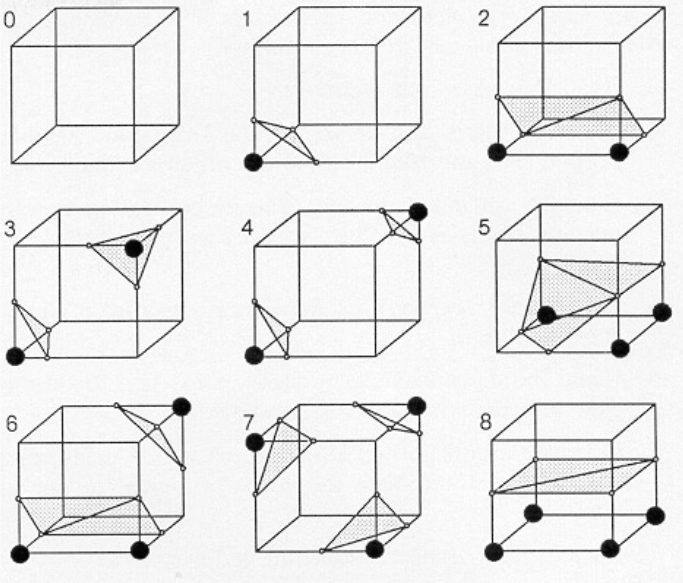
\includegraphics[width=1.0\textwidth]{imgs/base-cases-1.png}
          \end{center}
        \end{column}
        \begin{column}{0.48\textwidth}
          \begin{center}
            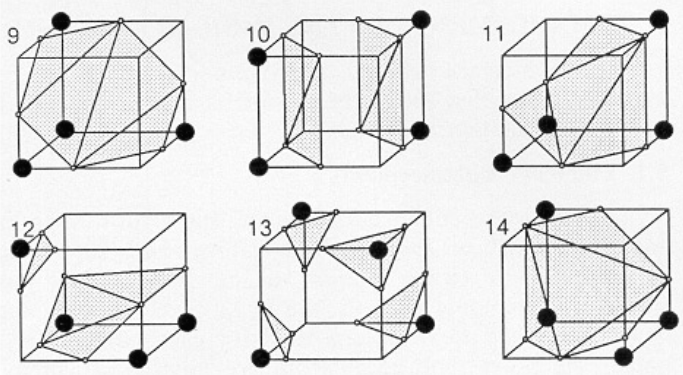
\includegraphics[width=1.0\textwidth]{imgs/base-cases-2.png}
          \end{center}
        \end{column}
      \end{columns}
    \end{frame}        

    \begin{frame}
      \frametitle{Casos complementares}
        \begin{itemize}
          \item Ambíguos
            \begin{center}
              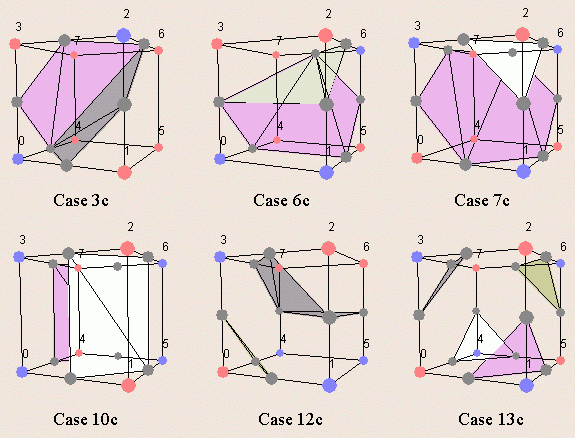
\includegraphics[width=.6\textwidth]{imgs/ambiguous-cases.png}
            \end{center}
        \end{itemize}
    \end{frame}        

    \begin{frame}
      \frametitle{Vantagens e desvantagens}
        \begin{itemize}
          \item Elimina a parametrização
          \item Visualmente satisfatório
          \item Nativo do PBRT
          \item Normais
          \item Muita memória
          \item Lento
        \end{itemize}
    \end{frame}        

  \section{Resultados}
  
    \subsection{}
    
      \begin{frame}
        \frametitle{Resultados}
        \begin{center}
          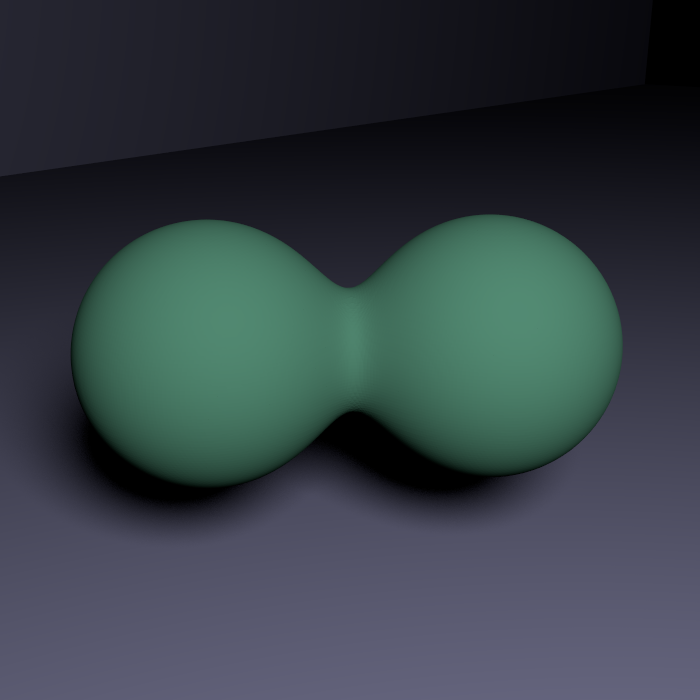
\includegraphics[width=.6\textwidth]{imgs/metaball-good1.png}
        \end{center}
      \end{frame}
  
      \begin{frame}
        \frametitle{Resultados}
        \begin{center}
          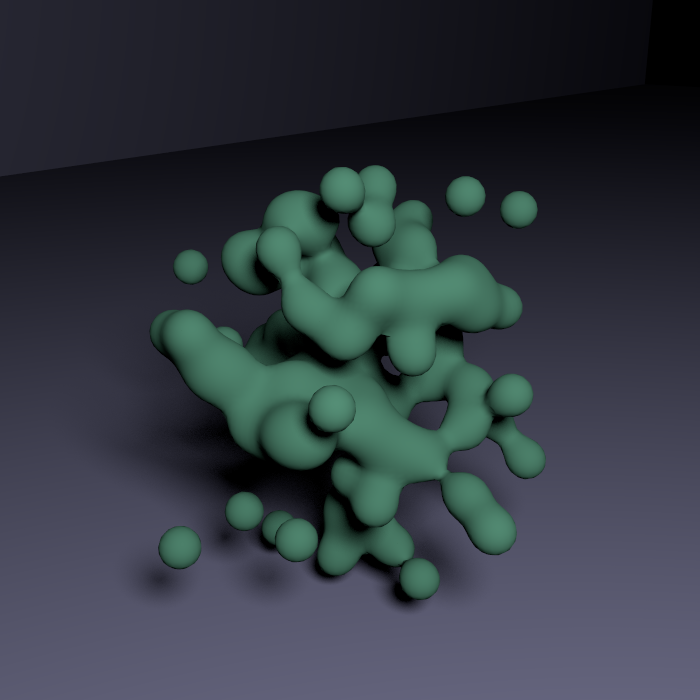
\includegraphics[width=.6\textwidth]{imgs/blob.png}
        \end{center}
      \end{frame}

      \begin{frame}
        \frametitle{Resultados}
        \begin{center}
          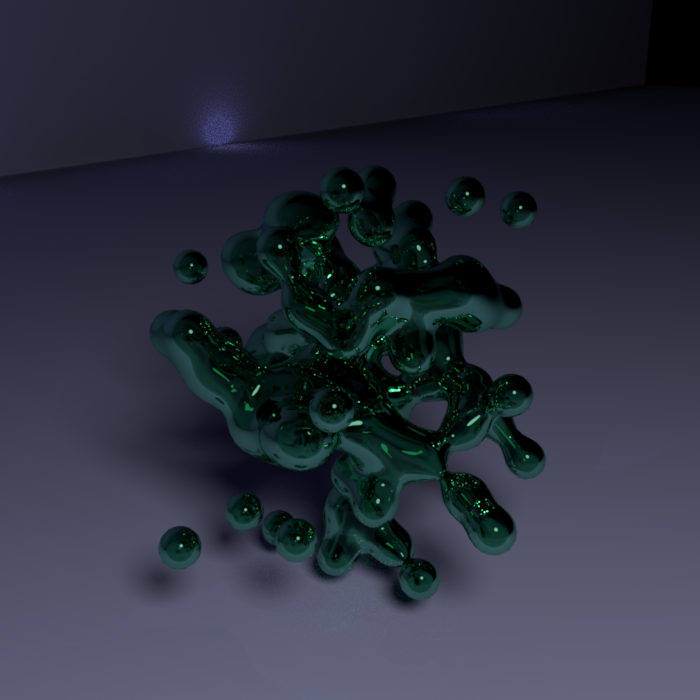
\includegraphics[width=.6\textwidth]{imgs/glass-blob-smooth.png}
        \end{center}
      \end{frame}

      \begin{frame}
        \frametitle{Resultados}
        \begin{center}
          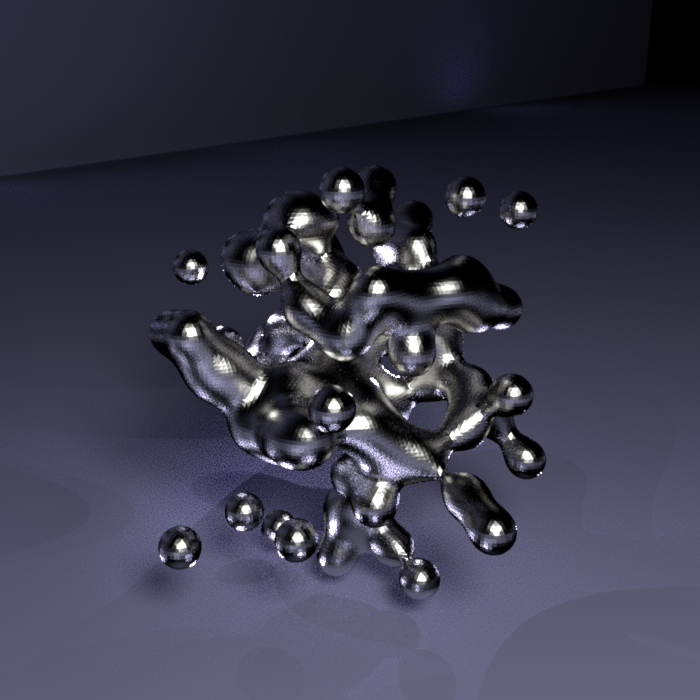
\includegraphics[width=.6\textwidth]{imgs/metal-blob.png}
        \end{center}
      \end{frame}

\section{Referências}
    \subsection{}
      \begin{frame}
        \frametitle{Referências}
        \begin{itemize}    
          \item BLINN, J. F. 1982. A generalization of algebraic surface drawing. \textit{SIGGRAPH Comput. Graph. 16}, 3 (July), 273–. 
          \item LORENSEN, W. E., AND CLINE, H. E. 1987. Marching cubes: A high resolution 3d surface construction algorithm. \textit{SIGGRAPH Comput. Graph. 21}, 4 (Aug.), 163–169.
          \item PHARR, M., AND HUMPHREYS, G. 2010. \textit{Physically Based Rendering, Second Edition: From Theory To Implementation}, 2nd ed. Morgan Kaufmann Publishers Inc., San Francisco, CA, USA.
        \end{itemize}
      \end{frame}

      \begin{frame}
        \frametitle{Referências}
        \begin{itemize}
          \item BLENDER-FOUNDATION, 2002-2014. Blender. \url{http://www.blender.org/}.
          \item INDUSTRIAL-LIGHT-\&-MAGIC, 2014. Openexr. \url{http://www. openexr.com/}.
          \item LINGRAND, D. The marching cubes. \url{http://users. polytech.unice.fr/~lingrand/MarchingCubes/algo.html}.
          \item GEISS, R. Metaballs (also known as: Blobs). \url{http://www.geisswerks.com/ryan/BLOBS/blobs.html}
        \end{itemize}
      \end{frame}

\end{document}
